\documentclass[12pt]{article}
\usepackage[utf8]{inputenc}
\usepackage{graphicx}
\usepackage{amsmath}
\usepackage{color}
\title{Producto 6 : Fuerza de Arrastre}
\author{Olga María Fimbres Morales}
\date{}
\begin{document}
\maketitle


 
 Todo objeto de masa m que se mueve a muy alta velocidad en un fluido de densidad P, experimenta una fuerza de arrastre FD contraria a la direccion de su movimiento y es dada por la ecuacion \\

donde u es la magnitud del vector velocidad el objeto, CD es el coeficiente de arrastre (adimensional), A es el area transversal presentada por el objeto. por ejemplo, para una esfera el area transversal es  , y el coeficiende de arrastre es CD = 0.47\\

Se pide agregar el efecto de resistencia del aire al objeto lanzada en tiro parabolico, El aobjeto ahora experimenta una fuerza de arrastre en la direccion del movimiento    o bien produciendo una aceleracion variable   .
\begin{center}
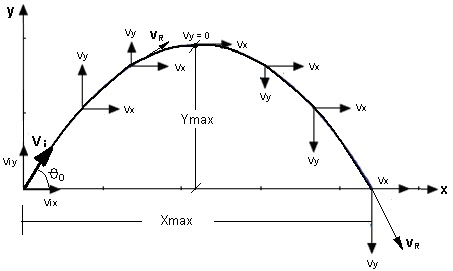
\includegraphics[scale=0.8]{Dibujo1.jpg}
\end{center}
\newpage
\begin{LARGE}
Estructura del código.
\end{LARGE}\\

\begin{large}
1.- Sección de declaración de constantes.
\end{large}\\
\\
Primeramente es necesario especificar las variables para un determinado escenario donde situaremos la simulación del tiro parabólico.\\ 
\\
En un inicio se utilizaron valores de densidad, gravedad y coeficiente de fricción para elavorar primeramenta un código que funcionara con estos valores, los cuales se posicionaron dentro de un modulo de constantes para que no fuera necesario especificarlos dentro de cada subrutina:
\begin{center}
\begin{verbatim}
module Cte
implicit none 
real, parameter :: g = 9.81, p =1.1644, pi = 4.0*atan(1.0), CD = 0.47
integer, parameter :: ntps=5000
end module Cte
\end{verbatim}
\end{center}

\begin{large}
2.- Sección de declaración de variables.
\end{large}\\
\\
En esta sección se especifican todas aquellas variables con las que va a trabajar el programa y con las que identificará cada elemento necesario para hacerlo. Primeramente, es necesario separarlas por cuales seran reales, cuales seran integrales y cuales utilizaras para realizar las operaciones dentro del DO. Y se escriben al inicio del programa y al inicio de las subrutinas.\\
\\
Algunas de las que se declaran como reales son definidas por operaciones realizadas con otros valores que se obtienen dentro del programa o bien dentro de las diferentes subrutinas y después son llamadas dentro de programa.



\begin{large}
3.- Subrutinas.
\end{large}\\
\\
Podemos realizar diferentes subrutinas dentro del programa que se encarguen de calcular diversas variables, las cuales podemos llamar dentro del programa para recoger sus valores y presentarlos como resultados.\\
En esta ocasión, se desarrollaron dos subrutinas, una que trabajara para calcular los resultados del tiro sin fricción y otra para el tiro con fricción.\\
Primeramente, la subrutina sin fricción, pide las siguientes variables:
\begin{verbatim}
subroutine Tiro_sfriccion(v0, dt_r, v0x, v0y, Xs, Ts, Ys, ttotal, xsf, ysf)
use Cte
\end{verbatim}
las cuales corresponden a la velocidad inicial, los grados en radianes, el ángulo convertido a radianes, la posicion final, el tiempo total de vuelo, la altura máxima alcanzada, y las variables que utilizaremos para realizar el LOOP, respectivamente.\\
En seguida corresponde ordenar las variables dependiendo de si seran solamente de entrada-intent(in)- o de entrada y salida -intent(inout)-. Tal como se muestra a continuación:
\begin{verbatim}
implicit none
real, intent(in) :: v0x, v0y, v0, dt_r
real, intent(inout) :: Xs, Ts, Ys, ttotal, xsf, ysf
real, dimension (0:ntps) :: xx, yy, tt
integer :: i
\end{verbatim}
Después, iniciamos el LOOP iniciando por abrir el archivo del cual graficaremos, y especificando desde donde iniciará y donde terminará los calculos:
\begin{verbatim}
open (1, file='tirosinfriccion.dat')
do i=0, ntps, 1
\end{verbatim}
Y las formulas que ya conocemos para el tiro parabólico sin fricción deben ser modificadas solamente en sus variables para que trabajen con los nuevos intervalos de tiempo que se han especificado, y señalando las conficiones bajo las que deseemos que trabaje, en este caso,se desea que trabaje solamente para valores positivos de Y.
\begin{verbatim}
 tt(i) = (float(i)*0.01)
  xx(i) = v0x*tt(i) 
  yy(i) = v0y*tt(i) - 0.5*g*tt(i)*tt(i)
write (1,*) xx(i), yy(i)
if (yy(i)<0) exit
end do
close (1)
\end{verbatim}
Finalmente, señalamos aquellos valores que llamaremos dentro del programa que seran nuestros resultados; para el tiempo total de vuelo y el alcanze máximo, basta con señalar el ultimo valor obtenido del LOOP, pero para obtener la altura máxima es necesario señalar que es ese el que deseamos con el comando Maxval, seguido de los arreglos a los que nos estamos refiriendo, el inicio de este y las confidiciones bajo las que trabaja.
\begin{verbatim}
ttotal =tt(i)
xsf = xx(i)
ysf = maxval(yy, 1, (yy(i)<0))
\end{verbatim}

\newpage
\begin{LARGE}
Análisis y evidencias.
\end{LARGE}
\\
Al comparar un tiro con una misma masa, velocidad inicial y ángulo, es posible darse cuenta de las claras diferencias entre un tiro parabólico en un modelo ideal y en un modelo real.\\
Como ejemplo de ello comparamos los tiros con y sin fricción de diversas parejas de ángulos complementarios.\\
\\
\begin{large}
10 y 80 grados.
\end{large}
\begin{center}
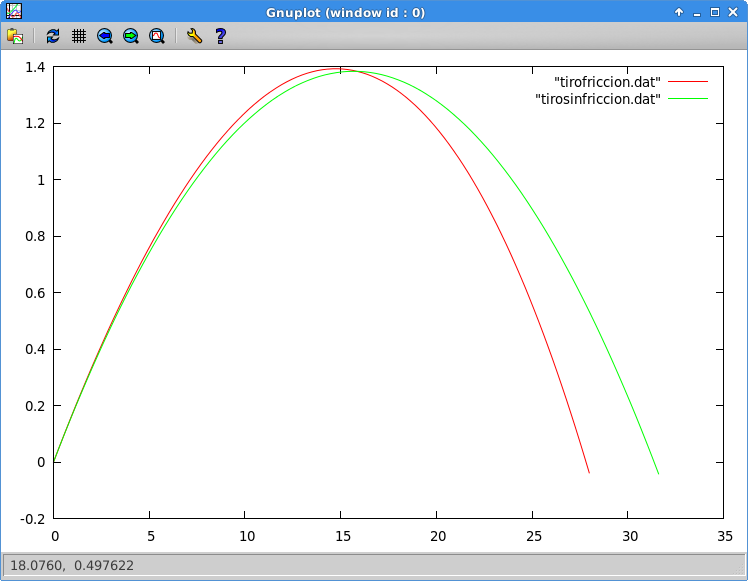
\includegraphics[scale=0.8]{producto610.png}
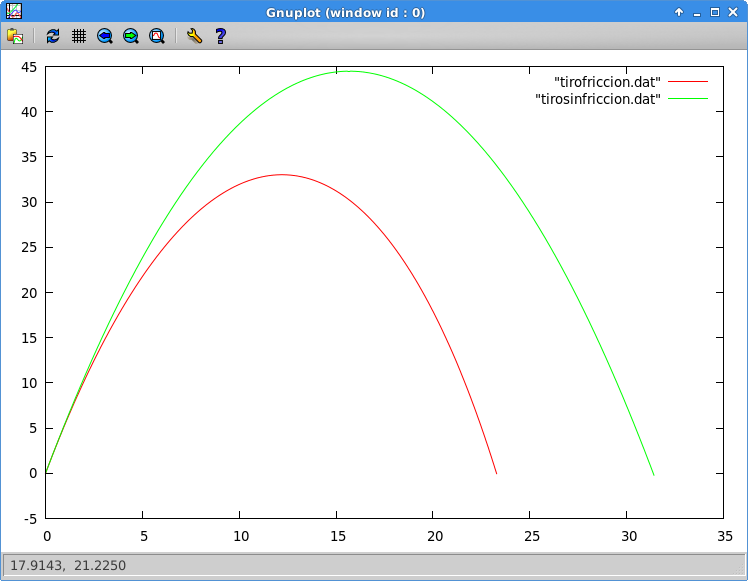
\includegraphics[scale=0.8]{producto680.png}
\end{center}
\begin{large}
20 y 70 grados.
\end{large}
\begin{center}
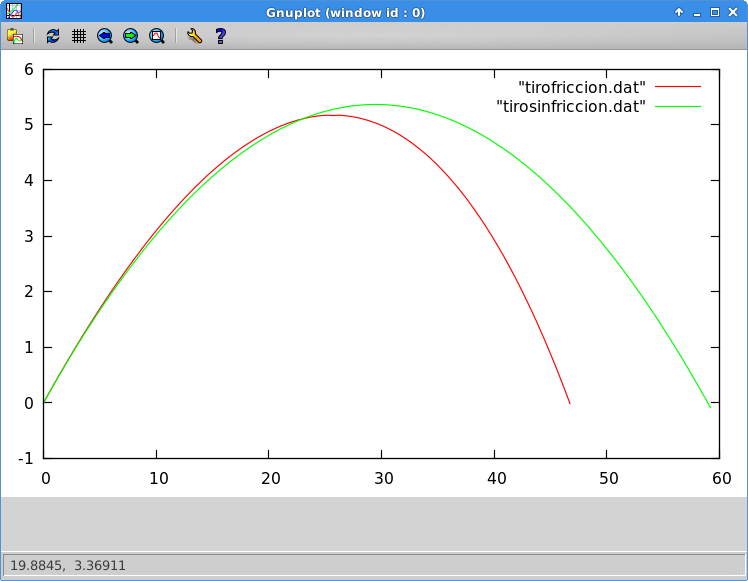
\includegraphics[scale=0.8]{producto620.png}
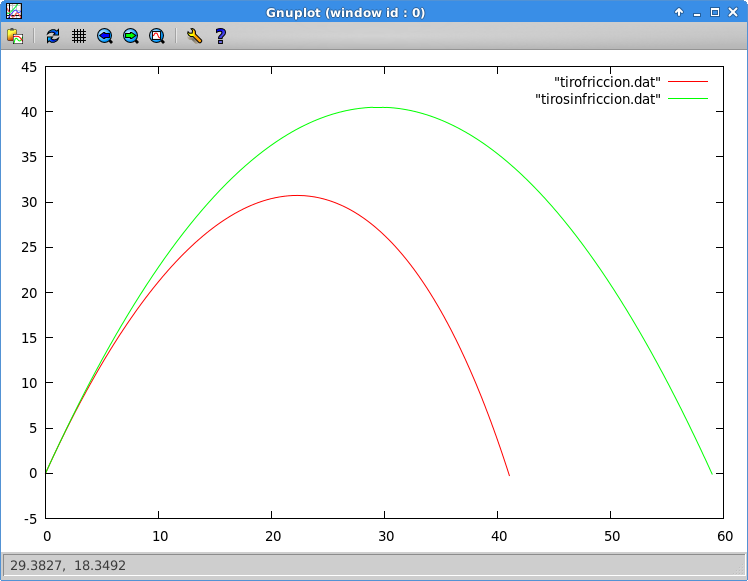
\includegraphics[scale=0.8]{producto670.png}
\end{center}
\begin{large}
30 y 60 grados.
\end{large}
\begin{center}
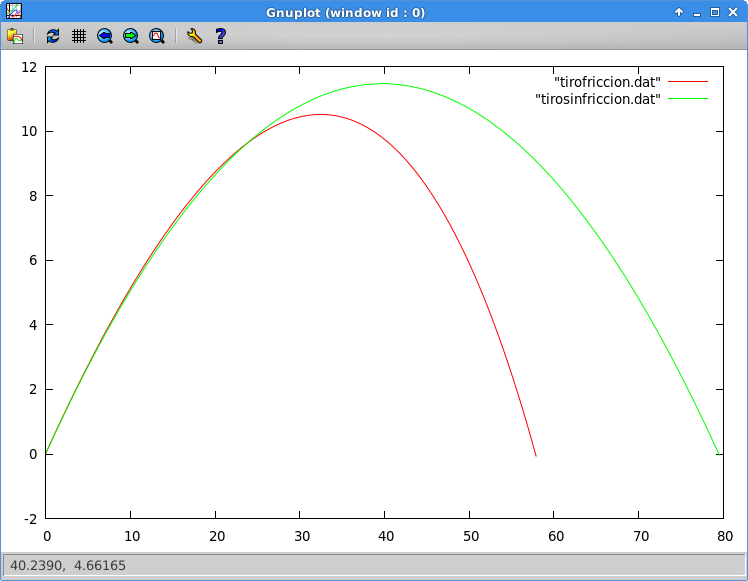
\includegraphics[scale=0.8]{producto630.png}
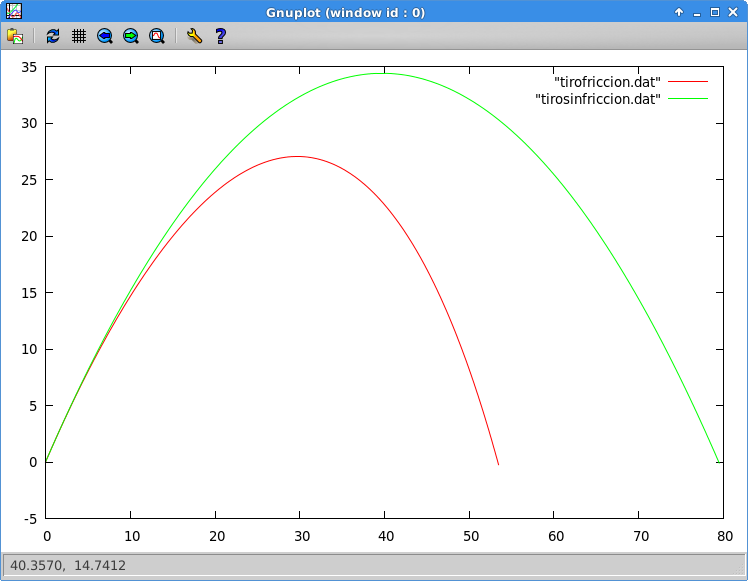
\includegraphics[scale=0.8]{producto660.png}
\end{center}
Finalmente, analizando estos resultados desde el punto de vista de la física, podemos darnos cuenta que el modelo real dista mucho del modelo ideal, ya que en el primero actuan más fuerzas que las que se consideran en el segundo; las cuales afectan los resultados del tiro.\\
Por ejemplo, al considerar la fricción del aire, podemos darnos cuenta que hay un punto en que al comparar las gráficas el tiro con fricción se encuentra sobre el tiro sin fricción, esto se debe a que en un mismo tiempo se encuentran en diferentes posiciones; en este caso, el tiro real se encuentra por detras del tiro ideal debido a la fuerza que ejerce el aire en el objeto, empujandolo hacia atras.\\
También podemos darnos cuenta que el tiempo que le toma subir alproyectil es mayor que el tiempo que le toma bajar, esto también debido a las fuerzas que actuan sobre el en cada etapa del tiro.
\newpage
\begin{LARGE}
Código.
\end{LARGE} 
\\

\begin{verbatim}
module Cte
implicit none 
real, parameter :: g = 9.81, p =1.1644, pi = 4.0*atan(1.0), CD = 0.47
! g = atiende al valor general que se le asigna a la gravedad terrestre, esta 
puede variar dependiendo de la altura o del planeta donde deseemos posicionar
la simulación.
!p = es la densidad del aire a una temperatura de 30 grados centigrados, 
la cual varia junto con la temperatura.
!CD = atiende al coeficiente de fricción de un cuerpo esférico, dependiendo 
del la forma del proyectil esta varia.
integer, parameter :: ntps=5000 ! este número solo atienda a la cantidad de 
puntos que se le desee poner como máximo para realizar las operaciones.
end module Cte

program Tiro_parabolico
use Cte
implicit none 
real :: dt, x0, y0, v0, v0x, v0y, m, dt_r, D, Xs, Ts, Ys, Xf, Tf, Yf, A, r,
ttotal, xsf, ysf, tt
real :: vxf(0:ntps), vyf(0:ntps), ax(0:ntps), ay(0:ntps), xx(0:ntps),
yy(0:ntps), ft(0:ntps), Vo(0:ntps)

print * , 'Datos iniciales'
write (*,*) 'Ingrese la masa del proyectil'
read *, m
print * , '-------------------------------------'
write (*,*) 'Identifique el radio del proyectil'
read *, r
print * , '-------------------------------------'
write (*,*) 'Ingrese una velocidad inicial para el proyectil'
read *, v0
print * , '-------------------------------------'
write (*,*) 'Ingrese un ángulo inicial para el proyectil'
read *, dt
print * , '-------------------------------------'
write (*,*) 'Determine una posición inicial en el eje x'
read *, x0
print * , '-------------------------------------'
write (*,*) 'Determine una posición inicial en el eje y'
read *, y0
print * , '-------------------------------------'

dt_r =(dt*pi)/180 !fortran trabaja las funciones trigonométricas con radianes,
asi que debemos convertir los grados a radianes. 
v0x = v0*cos(dt_r) !velocidad inicial en x.
v0y = v0*sin(dt_r) !velocidad inicial en y.
A = pi*r*r !area transversal .
D = p*CD*A*0.5 !constante de fricción.

print * , '-------------------------------------'
print * , '-------------------------------------'
print * , '-------------------------------------'
print * , '-------------------------------------'
print * , '-------------------------------------'

call Tiro_sfriccion(v0, dt_r, v0x, v0y, Xs, Ts, Ys, ttotal, xsf, ysf) 
!llamamos a la subrutina pertinente para que 
nos muestre los valores que estamos pidiendo.
print * , 'Modelo Ideal'
print * , 'Tiempo de vuelo', ttotal, 'segundos'
print * , 'Alcance', xsf, 'metros'
print * , 'Altura máxima', ysf, 'metros'
print * , '-------------------------------------'
print * , '-------------------------------------'
print * , '-------------------------------------'
call Tiro_friccion1(v0, v0x, v0y, ax, ay, Xf, Tf, Yf, x0, y0, vxf, vyf, ft, D, 
m, Vo) !llamamos a la subrutina.
print * , 'Modelo real'
print * , 'Tiempo de vuelo',Tf ,'segundos'
print * , 'Alcance',Xf ,'metros'
print * , 'Altura máxima',Yf ,'metros'
end Program Tiro_parabolico

subroutine Tiro_sfriccion(v0, dt_r, v0x, v0y, Xs, Ts, Ys, ttotal, xsf, ysf)
use Cte
implicit none
real, intent(in) :: v0x, v0y, v0, dt_r
real, intent(inout) :: Xs, Ts, Ys, ttotal, xsf, ysf
real, dimension (0:ntps) :: xx, yy, tt
integer :: i

Ts = 2*v0*sin(dt_r)*(1/g)
Ys = v0*v0*sin(dt_r)*sin(dt_r)*(1/(2*g))
Xs = v0*v0*sin(2*dt_r)*(1/g)

open (1, file='tirosinfriccion.dat')
do i=0, ntps, 1
  
  tt(i) = (float(i)*0.01)
  xx(i) = v0x*tt(i) 
  yy(i) = v0y*tt(i) - 0.5*g*tt(i)*tt(i)
write (1,*) xx(i), yy(i)
if (yy(i)<0) exit
end do
close (1)

ttotal =tt(i)
xsf = xx(i)
ysf = maxval(yy, 1, (yy(i)<0))

end subroutine Tiro_sfriccion

subroutine Tiro_friccion1(v0,v0x, v0y, ax, ay, Xf, Tf, Yf, x0, y0, 
vxf, vyf, ft, D, m, Vo) 
use cte
implicit none
real, intent(in) :: v0, v0x, v0y, x0, y0, D, m
real, intent(inout) :: Xf, Tf, Yf
real, dimension (0:ntps) :: fx, ft, fy, vxf, vyf, ax, ay, Vo
integer :: i
   
   fy = 0
   ft(0)=0
   fx(0)=x0
   fy(0)=y0
   vxf(0)=v0x
   vyf(0)=v0y
   ax(0) = -(D/m)*(v0x)*(v0x)
   ay(0) = -g - ((D/m)*(v0y)*(v0y))

open (2, file='tirofriccion.dat')  
do i = 0, ntps, 1

ft(i+1) = (ft(i)*0.01) +0.01 !Intervalo de tiempo
vxf(i+1) = vxf(i) + (ax(i)*ft(i+1))!Velocidad X
vyf(i+1) = vyf(i) + (ay(i)*ft(i+1)) !Velocidad Y.
fx(i+1) = fx(i) + (vxf(i)*ft(i+1)) + ((1/2)*ax(i)*ft(i+1)*ft(i+1)) !Posición X.
fy(i+1) = fy(i) + (vyf(i)*ft(i+1)) + ((1/2)*ay(i)*ft(i+1)*ft(i+1)) !Posición Y.
ax(i+1) = -(D/m)*(vxf(i))*(vxf(i)) !Aceleracion X.
ay(i+1) = -g - ((D/m)*(vyf(i))*(vyf(i))) !Aceleración Y

write (2, 1001) fx(i), fy(i)
if (fy(i)<0) exit !Condición.
end do
1001 format (2f10.6)
close (2)
<<<<<<< HEAD
velx= vxf(i)
vely= vyf(i)
acely= ay(i)
acelx= ax(i)
Tf = ft(i)
Xf = fx(i)

!Últimos valores encontrados y el máximo valor de Y.
Tf = ft(i) * 10.0
Xf = fx(i+1)
Yf = maxval(fy, 1, (fy(i)<0))
end subroutine Tiro_friccion1
\end{verbatim}
\end{document}